\documentclass[tikz,border=6pt]{standalone}
\usepackage{amsmath}
\usepackage{xcolor}

\definecolor{blockblue}{HTML}{4A90D9}

\begin{document}
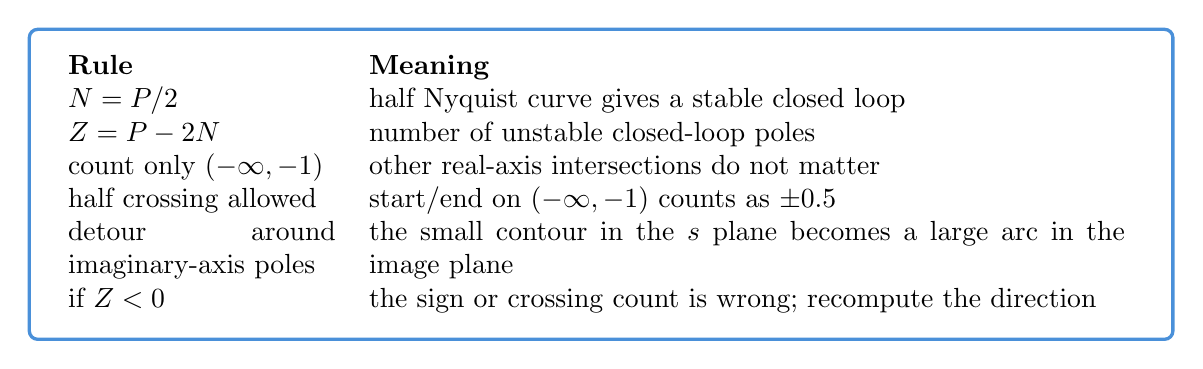
\begin{tikzpicture}[line width=1.2pt]
  \node[
    draw=blockblue,
    rounded corners=3pt,
    inner sep=8pt,
    align=left
  ] at (0,0) {
    \begin{tabular}{p{3.4cm}p{9.6cm}}
      \textbf{Rule} & \textbf{Meaning} \\
      $N=P/2$ & half Nyquist curve gives a stable closed loop \\
      $Z=P-2N$ & number of unstable closed-loop poles \\
      count only $(-\infty,-1)$ & other real-axis intersections do not matter \\
      half crossing allowed & start/end on $(-\infty,-1)$ counts as $\pm 0.5$ \\
      detour around imaginary-axis poles & the small contour in the $s$ plane becomes a large arc in the image plane \\
      if $Z<0$ & the sign or crossing count is wrong; recompute the direction \\
    \end{tabular}
  };
\end{tikzpicture}
\end{document}
